% -------------------------------------------------------------------------------------------------
% SOLUTION ARCHITECTURE
% -------------------------------------------------------------------------------------------------
\section{Cloud4Things}
\label{sec:solution}
Cloud4Things is a solution that automates the provisioning of software for Internet of Things
applications in the cloud. Our solution relies on configuration management tools that leverage
existing software stacks - e.g RFID software. In Figure \ref{fig:c4t_architecture} we present
the architecture of Cloud4Things.
% Automatic provisioning diagram
\begin{figure}[!ht]
  \centering
  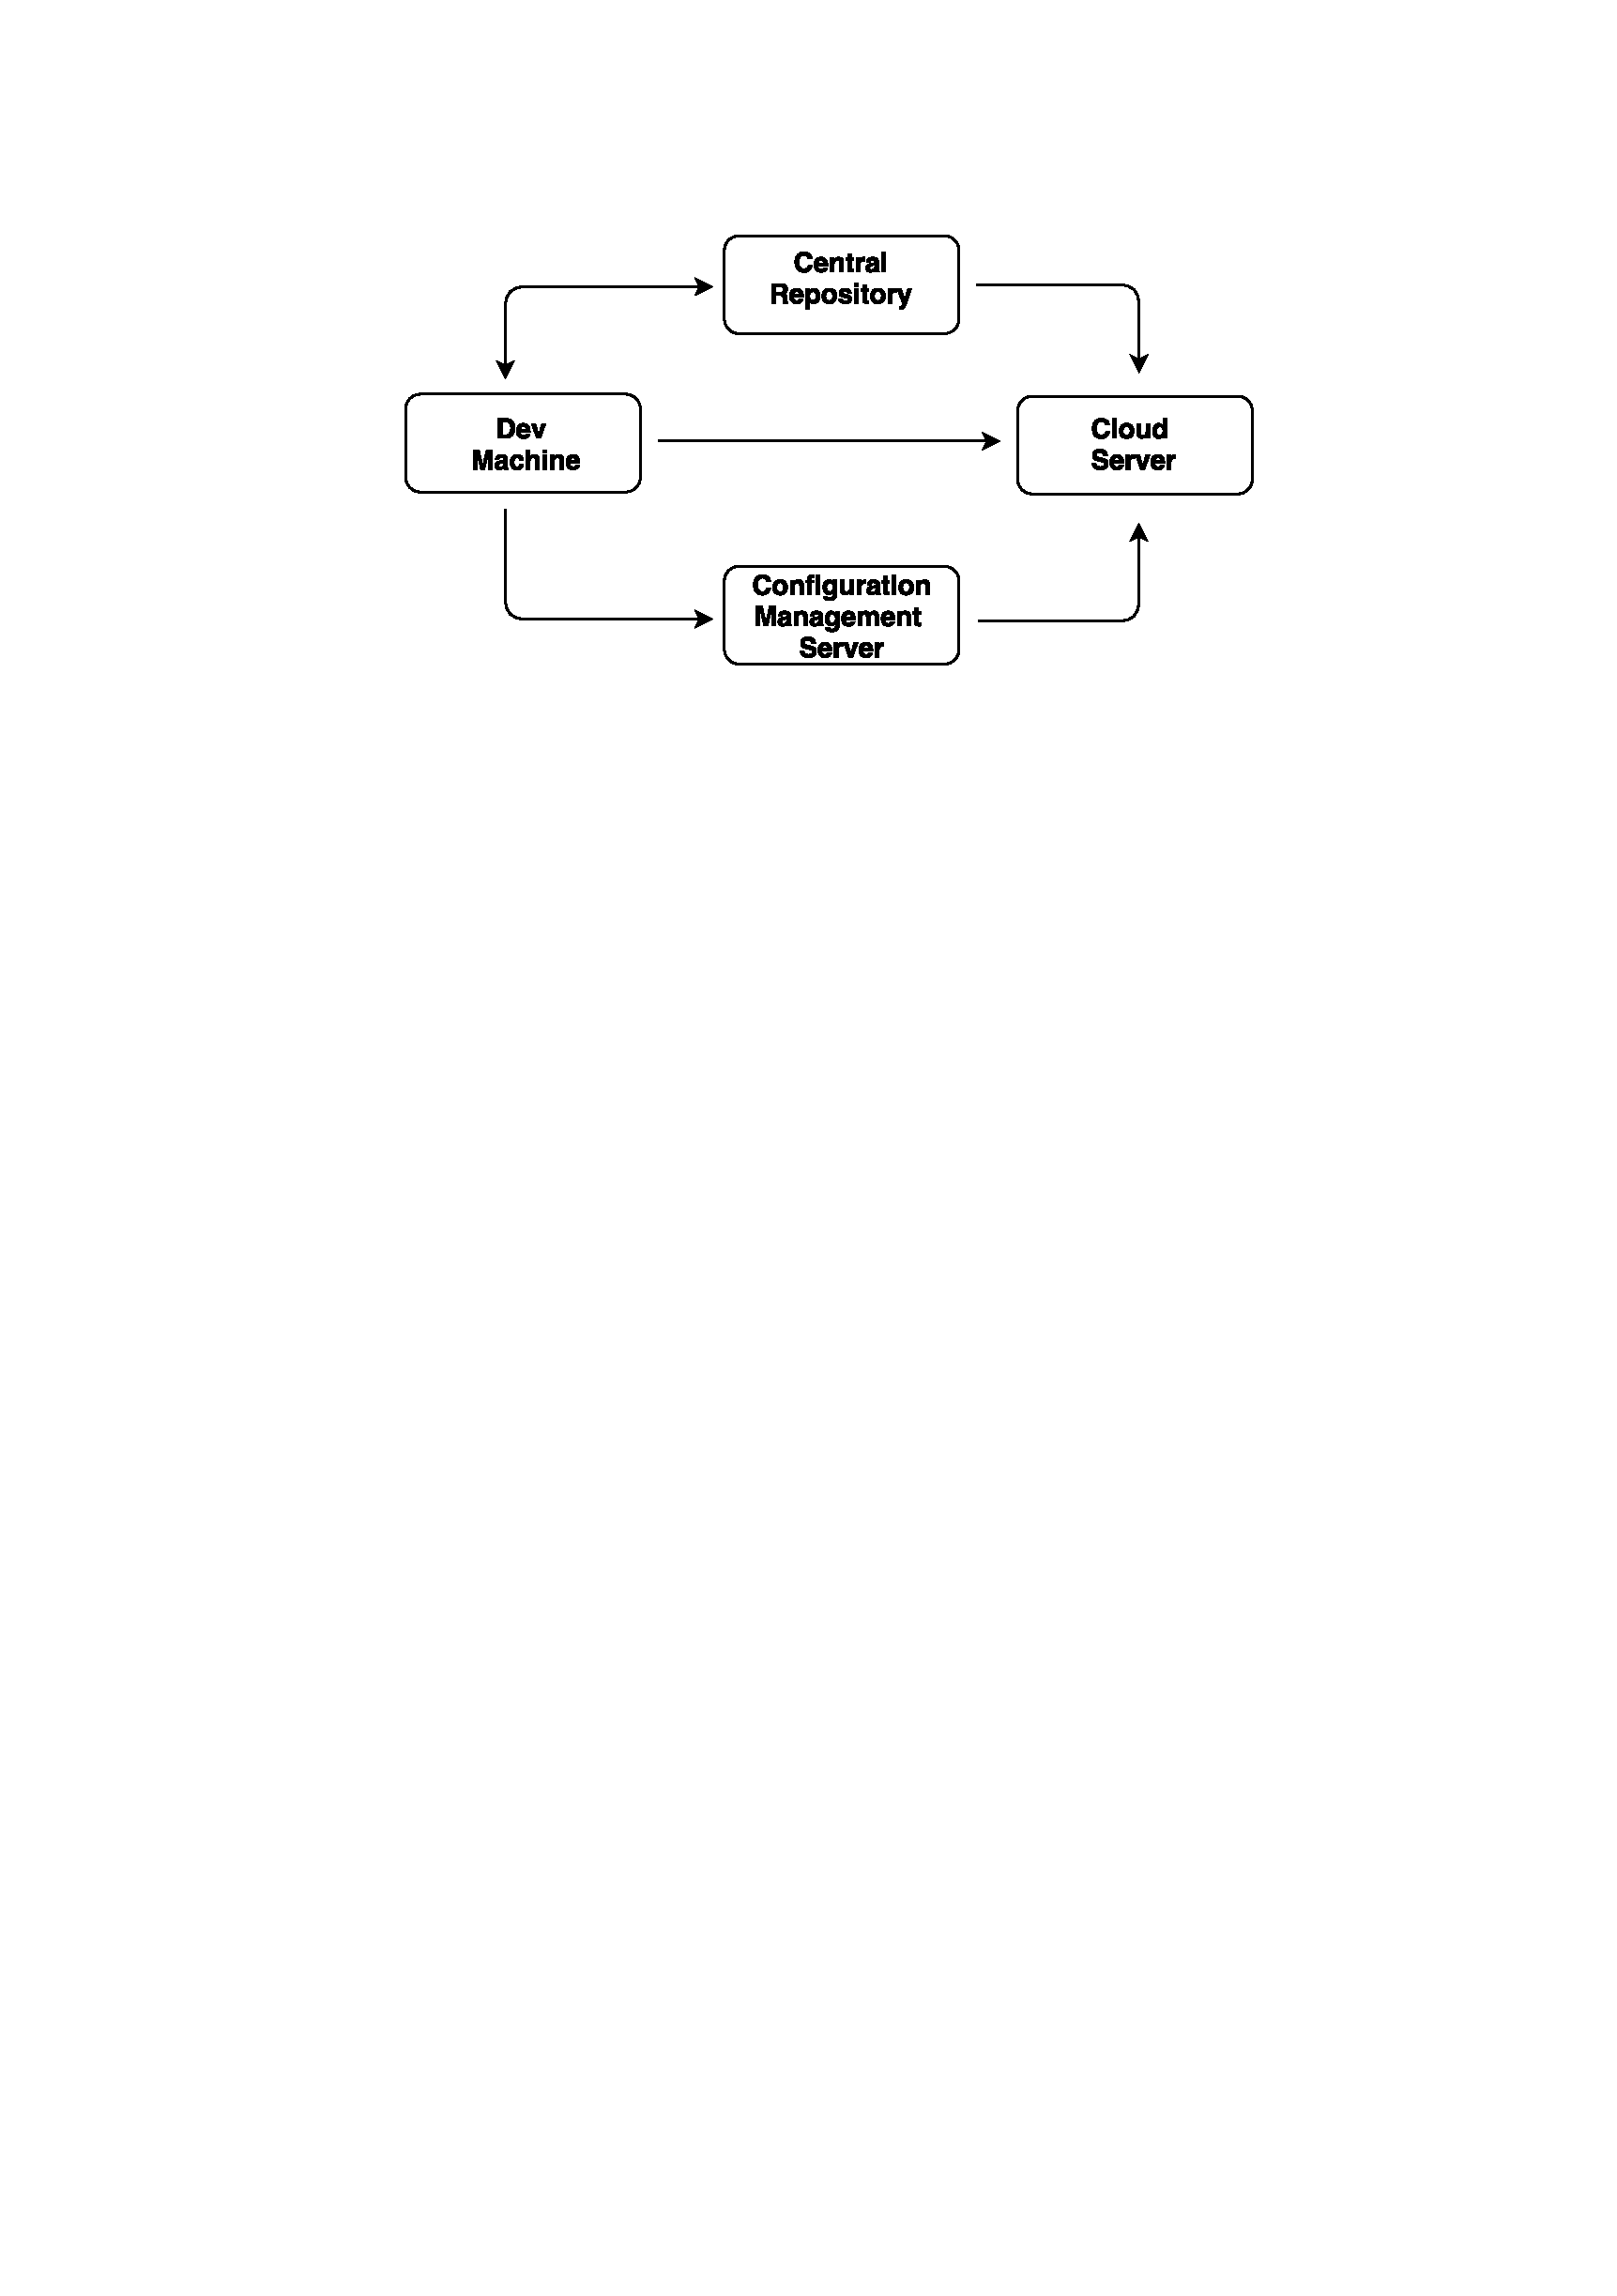
\includegraphics[width=.7\textwidth]{images/c4t-generic-solution.pdf}
  \caption{Cloud4Things conceptual architecture.}
  \label{fig:c4t_architecture}
\end{figure}

In our architecture, the provisioning policies and software images of a smart place are defined and configured
in a local environment and then uploaded to its respective repositories. When the provisioned request
is performed - through a configuration management interface in a local environment - the configuration
management (CM) client in the server node pulls the polices from the configuration management server,
a centralized server that is responsible to maintain a consistent state of the provisioned nodes in
the cloud. In order to enforce the polices, the CM client pulls the software images from a central
repository and then performs the provisioning and configuration of the software. After provisioning
the infrastructure the CM client periodically polls the CM server in order to determine if its current
state is consistent with the most recent policy.

\subsection{Implementation}
\label{sub:implementation}
% -------------------------------------------------------------------------------------------------
% CHEF AUTOMATIC PROVISIONING
% -------------------------------------------------------------------------------------------------
The current implementation of Cloud4Things relies on the Chef\footnote{https://www.chef.io/} tool.
The \textit{recipes} that describe our infrastructure are based on \textit{cookbooks} that are available on the
Chef Supermarket\footnote{https://supermarket.chef.io/}. These \textit{recipes} describe how our software stack -
are provisioned in the cloud instances. In our current prototype, we will use Docker containers to provisioning
the smart place software and we chose to use Amazon Web Services as cloud provider. To provisioning the
resources in the Amazon EC2 instances we will use \textit{knife}, a command-line tool developed by Chef that provides
an interface between a local Chef repository and the Chef server. The provisioning workflow is illustrated
in Figure \ref{fig:automatic_provisioning}.
% Automatic provisioning diagram
\begin{figure}[!ht]
  \centering
  \makebox[\textwidth][c]{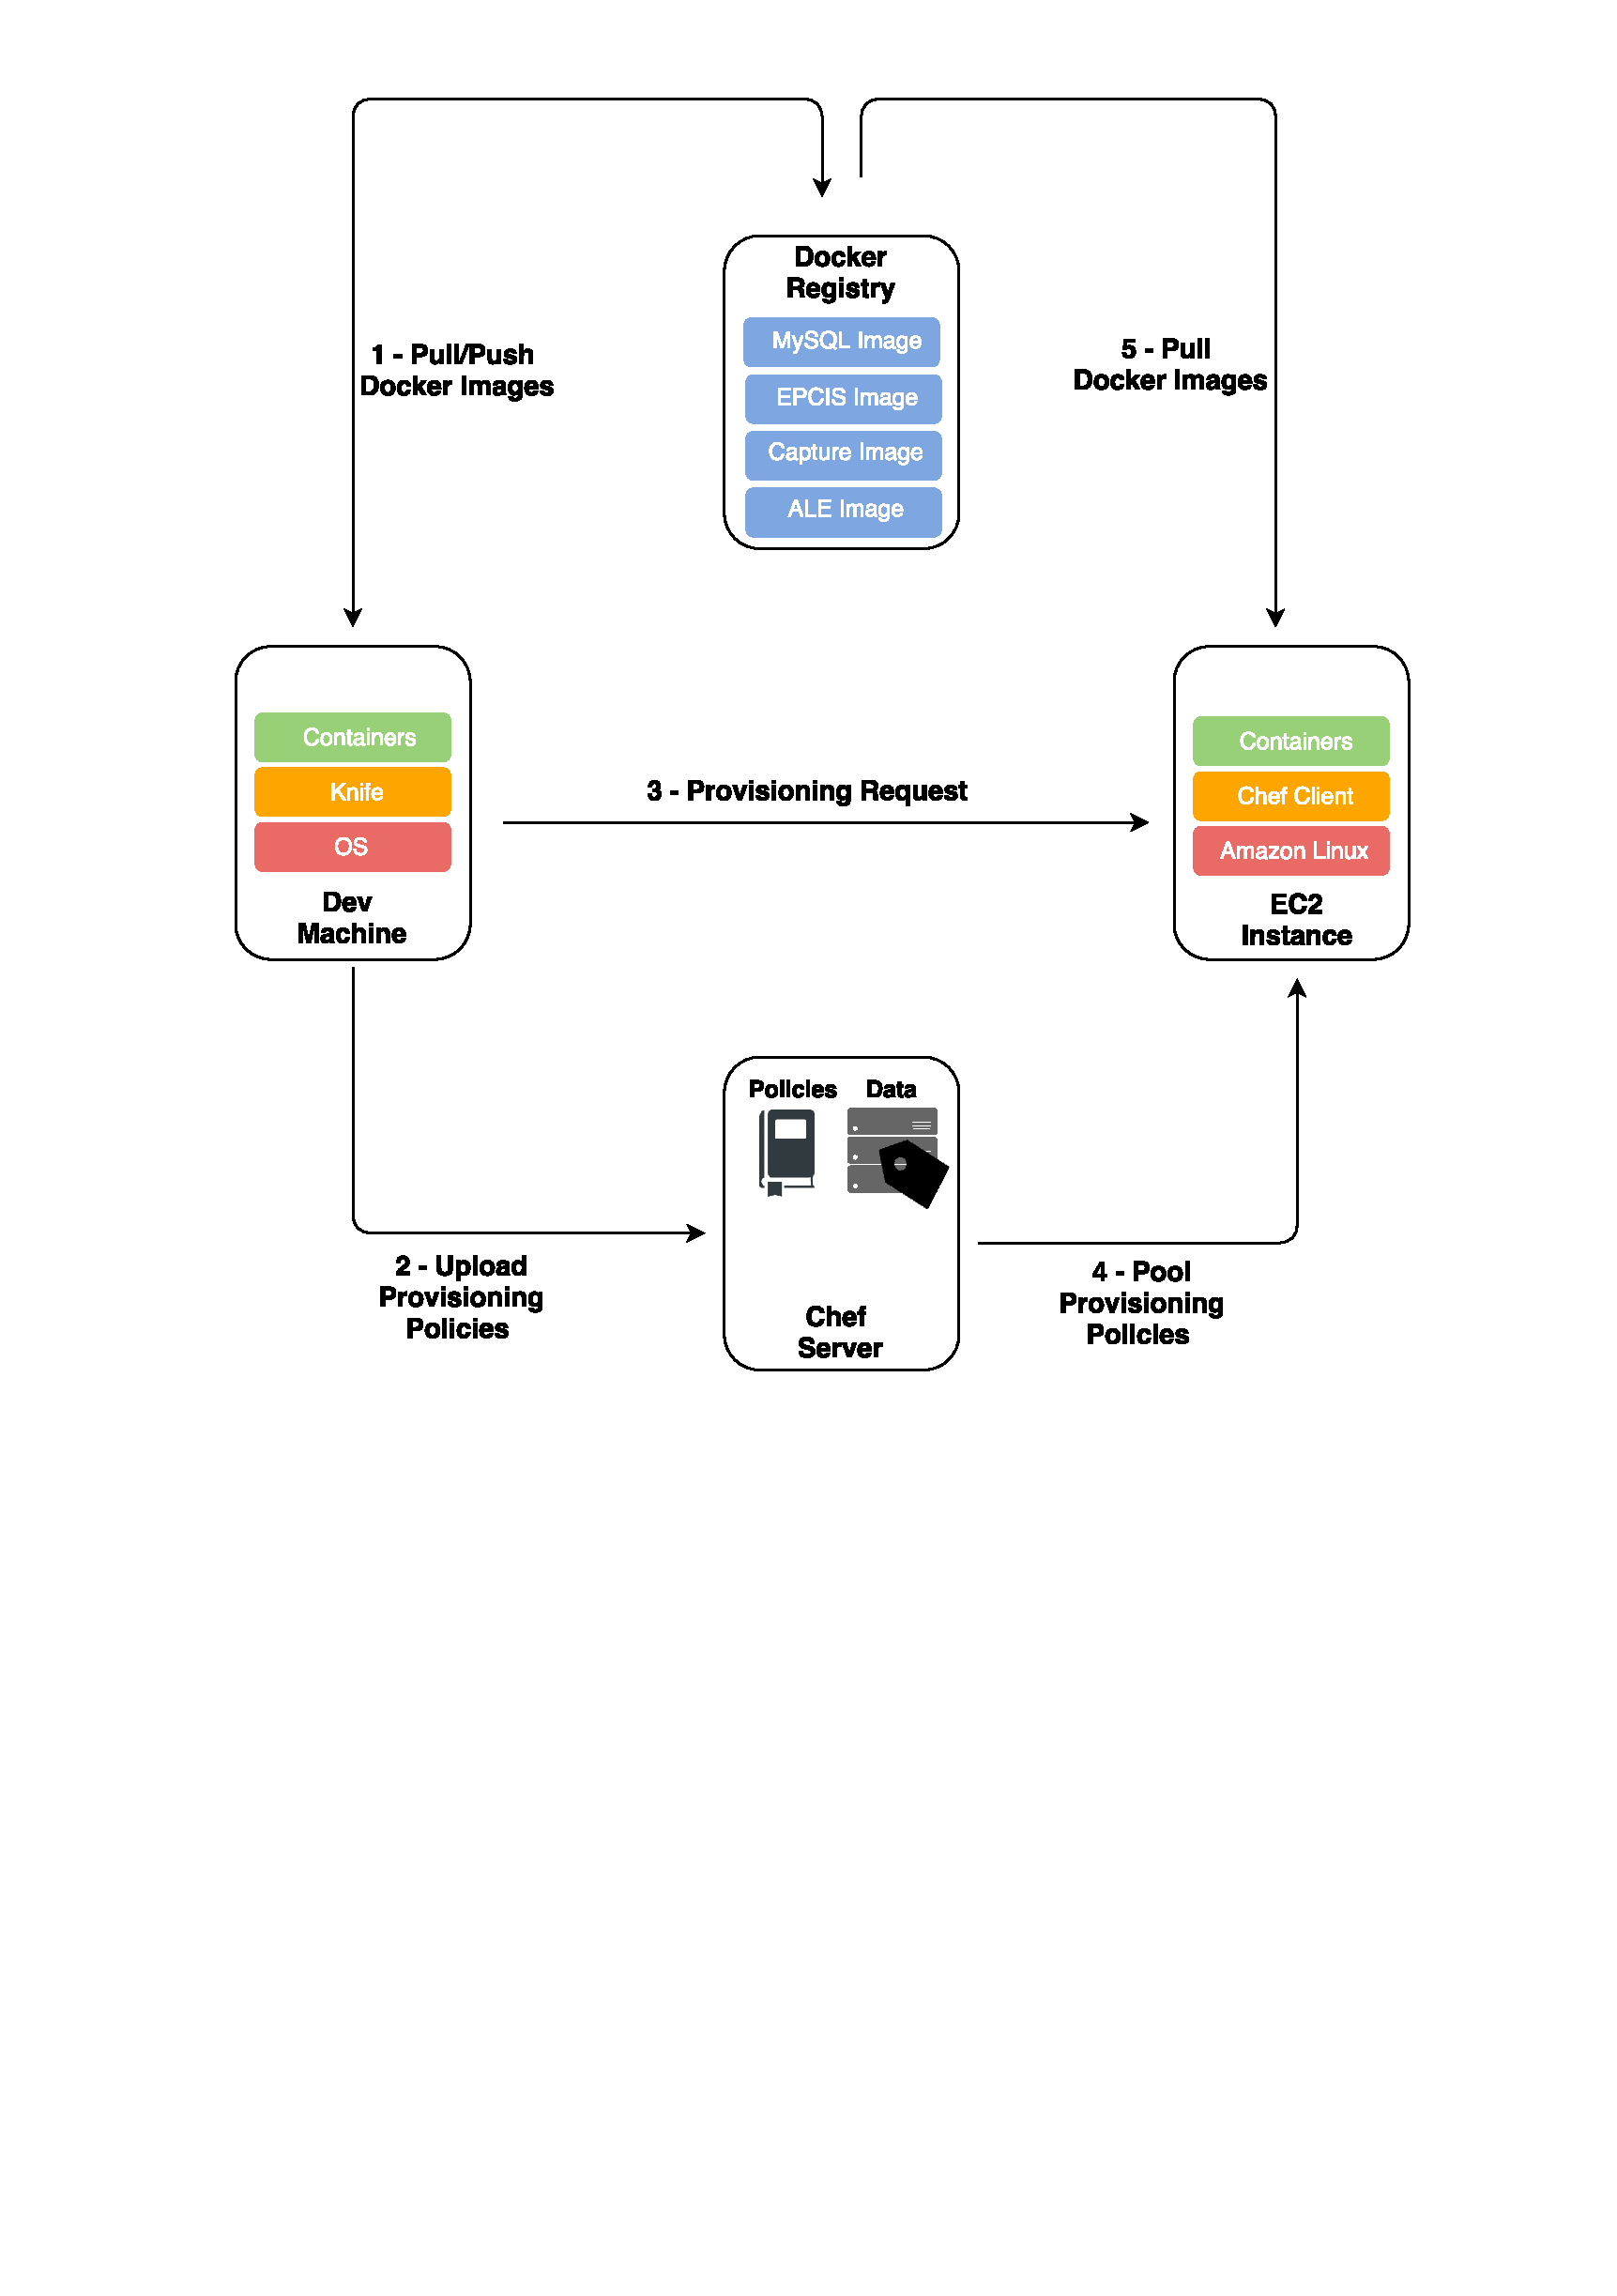
\includegraphics[width=\textwidth]{images/c4t-tech-architecture}}%
  \caption{Automatic provisioning workflow.}
  \label{fig:automatic_provisioning}
\end{figure}

In a development environment the Docker images are built and then uploaded to the Docker Registry
repository (1). The provisioning of the cloud resources is described in the cookbooks that are uploaded
to the Chef server (2). The provisioning request (3) is performed using knife - knife has a plugin for EC2
that allows to describe the image type, the instance type and the policies that need to be applied on
each provisioned node. Then the Chef client runs the configuration recipes that are pulled from the Chef server (4).
In our solution these configuration recipes describe that our nodes must have a set of Docker containers
running on it. The Chef client pulls the Docker images from the remote repository, build the
containers based on those images and finally applies the configuration that is associated to each container.

% -------------------------------------------------------------------------------------------------
% Containers
% -------------------------------------------------------------------------------------------------
\subsubsection{Containers}
\label{subs:containers}
Docker\footnote{https://www.docker.com} is an open source project to pack, ship and run any application
as a lightweight container. Docker containers are \textit{hardware-agnostic} and \textit{platform-agnostic},
this means that these containers can run anywhere, from a laptop to a EC2 compute instance. Since Docker
is based in Linux Containers (LXC), the virtualization is performed at operating-system level, different of
hypervisor-based solutions where the virtualization is performed at hardware-level. While the effect of both
types of virtualization are similar, the virtualization at the operating-system level provides significant
benefits compared to hypervisor-based solutions\cite{Merkel}. Docker containers are small, they have low
memory and CPU overhead, they also are portable between different virtualization environments.

In our solution, Docker containers are used to provisioning the software stack of the Fosstrak platform.
A complete installation of Fosstrak requires a compatible Java SDK, a full MySQL database and
a Apache Tomcat server. In order to improve the application scalability we are provisioning a single container
for each component of the Fosstrak platform, the EPCIS repository, the Capture application, the ALE server,
and also for the MySQL database.

By default each container runs a process that is isolated from the other processes that are executed in
the same environment. In order to connect the different modules of the Fosstrak, our containers are
linked through the \textit{linking} mechanism provided by Docker. Another benefit that the Docker platform
provides is the Docker Registry service, a public repository that stores Docker images used to create the
containers. In our solution we built the Docker images of the Fosstrak modules and published them
in Docker registry to later be used to create our containers.
% -------------------------------------------------------------------------------------------------
% Configuration Management Tools
% -------------------------------------------------------------------------------------------------
\subsubsection{Configuration Management Tools}
\label{subs:cm_tools}
Chef is a configuration management tool that allows to describe the infrastructure as code. In that way
it is possible to automate how the infrastructure is built, deployed and managed.

Chef architecture is composed of the Chef Server - that stores the recipes and other configuration data -
and the  Chef Client - that is installed in each server, VM or container, i.e, the nodes that are managed with Chef.
The Chef client periodically polls Chef server latest policy and state of the network, and if anything on the
node is out of date, the client update its state in order to be consistent with the latest policy.

Chef was built from the ground with the cloud infrastructure in mind. With Chef, is possible to dynamically
provision and de-provision the application infrastructure on demand to keep up with peaks in usage and traffic.
For instance, Chef offers several plugins for provisioning cloud resources in different hosts such as
Amazon EC2, Google Compute Engine and OpenStack.
